\section{Reading the leaderboard}
\label{sec:lb}

\subsection{The ladder, and why CV under-predicts the gain}
Table~\ref{tab:blends} and Figure~\ref{fig:progress}b tell one coherent story. Every model sits
about \dlt{3} below its cross-validated score --- the offset is remarkably stable
($-2.6$, $-3.1$, $-3.6$ \dlt{} across versions), which is what an exchangeable split predicts.
What changes is the \emph{slope}: the same $+1.0$ \dlt{} of cross-validated improvement is worth
$+0.1$ \dlt{} when it comes from seed averaging, $+0.6$ when it comes from a three-family blend,
$+1.3$ when it comes from seven families and $+1.5$ when the FT-Transformer joins. Averaging
different \emph{functions} generalises better than averaging one function many times, and the
public split (299{,}844 rows) sees that more clearly than five validation folds of 140{,}000
rows each.

The counter-example is equally instructive: three-seeded FT-Transformer is the best
cross-validated model we built (0.960942) but scored 0.96061, one $10^{-5}$ below its
single-seeded sibling. We therefore kept the leaderboard-best artifact and recorded both
numbers in the model-selection file. Reporting the CV-best number while shipping the LB-best
file would have been the easy way to make this section look better than it is.

\subsection{What the leaderboard's shape implies}
Figure~\ref{fig:rank} converts the remaining gap into effort: near our band roughly 50 places
cost $10^{-4}$ of \auc{}, so the 1.1 \dlt{} that separate us from the top decile (0.96192) is
about 550 places. Two further observations from the snapshot of 3{,}061 teams help calibrate
what such a jump would require.

First, the board is dominated by ties. Of 3{,}013 teams in an earlier snapshot only 749 distinct
scores exist, and 130 teams share the single value 0.96213 (ranks 21--150). A 130-way tie at
five decimals is not 130 independent discoveries; it is the signature of a shared artifact ---
published out-of-fold predictions and frozen stacks, which are explicitly distributed in this
competition. Second, submission counts increase with rank: the median top-10 team has made 47
submissions against 4 for the field, and the top two have made 178 and 150. Because the public
board records a team's best public submission, part of the visible gap is selection, not skill;
the private split will settle it.

Finally, the two leaders are outliers in a way that stacking arithmetic does not explain:
$+0.64$ \dlt{} above rank 2 and $+1.04$ \dlt{} above rank 3, whereas ranks 3--10 span only
$0.32$ \dlt{}. We could not identify the mechanism from public material, and we ruled out the
leak candidates we could test (Section~\ref{sec:leak}).

\begin{figure}[t]
\centering
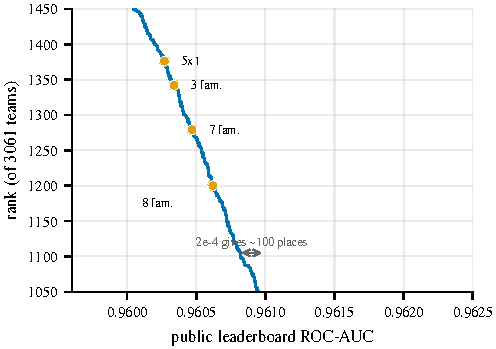
\includegraphics[width=0.68\linewidth]{figures/fig_rank.pdf}
\caption{Public leaderboard rank against score, zoomed on the band around our submissions.
Near this score, \dlt{2} of \auc{} buys roughly one hundred places; the top decile is
1.1 \dlt{} away.}
\label{fig:rank}
\end{figure}
